\ifpdf
    \graphicspath{{Appendix1/}}
\else
    \graphicspath{{Appendix1/}}\fi

\let\svaddcontentsline\addcontentsline
\renewcommand\addcontentsline[3]{%
  \ifthenelse{\equal{#1}{lof}}{}%
  {\ifthenelse{\equal{#1}{lot}}{}{\svaddcontentsline{#1}{#2}{#3}}}}

\chapter{PHỤ LỤC 1: Quản lý dữ liệu trên Firebase	}
{\Large \textbf{Giới thiệu về Firebase }}
\begin{itemize}
	\item \textbf{Realtime Database}
	\item [] \textbf{Chia sẻ tài nguyên giữa các thiết bị: }Cơ sở dữ liệu thời gian thực trên Firebase lưu trữ dữ liệu dưới dạng NoSQL, cho phép người dùng lưu trữ và đồng bộ thời gian thực với mọi thiết bị đầu cuối. Tất cả các thiết bị điện thoại, website..v..v... kết nối đến Firebase đều chia sẻ một cơ sở dữ liệu Firebase duy nhất và luôn luôn tự động cập nhập dữ liệu mới nhất.
	\item [] \textbf{Xây dựng ứng dụng không cần server: }Sử dụng bộ SDK cung cấp bởi Google, người dùng sẽ không cần tốn công sức bỏ ra cho việc thiết lập server của riêng mình nữa. Thậm chí, người dùng còn có khả năng cài đặt code backend và triển khai ngay trên Firebase. Các máy chủ của Firebase quản lý hàng triệu kết nối đồng thời và hàng tỉ lượt truy vấn mỗi tháng luôn sẵn sàng phục vụ người dùng.
	\item [] \textbf{Tối ưu hoá cho làm việc offline: }Khi người dùng không kết nối Internet, Firebase sẽ phát hiện và chuyển sang sử dụng cache trên thiết bị để lưu trữ thay đổi của người dùng. Khi thiết bị được kết nối Internet trở lại, dữ liệu lưu trên cache được tự động đồng bộ với máy chủ Firebase.
	\item[] \textbf{Bảo mật người dùng tốt: }Tất cả dữ liệu được truyền qua một kết nối an toàn SSL với một chứng nhận 2048-bit. Cở sở dữ liệu truy vấn và việc xác nhận  được điều khiển tại một cấp độ chi tiết sử dụng theo một số các quy tắc mềm dẻo security rules language.  Tất cả các logic bảo mật dữ liệu của bạn được tập trung ở một chỗ để dễ dàng cho việc cập nhật và kiểm thử.\\[0.01cm]
	\item \textbf{Firebase Authentication}
	\item [] Sử dụng Firebase, người dùng có thể dễ dàng xây dựng chức năng xác thực người dùng.Firebase cung cấp xác thực người dùng với Email, Facebook, Twitter, GitHub, Google, và xác thực nạc danh Firebase đã xây dựng chức năng cho việc xác thực người dùng với Email, Facebook, Twitter, GitHub, Google, và xác thực nạc danh.\\
\end{itemize}

{\Large \textbf{Làm việc với giao diện console quản lý}}
\begin{itemize}
	\item Truy cập vào đường dẫn \url{https://console.firebase.google.com/}
	\item Đăng nhập với thông tin sau đây:
	\item [] \indent{Tài khoản: }eslrecommend.manager@gmail.com
	\item [] \indent{Mật khẩu: }eslrecommend2017
	\item Chọn ứng dụng "ESLRecom" và truy cập vào màn hình quản lý của Firebase  
\begin{figure}[H]
  \begin{center}
    %\leavevmode
    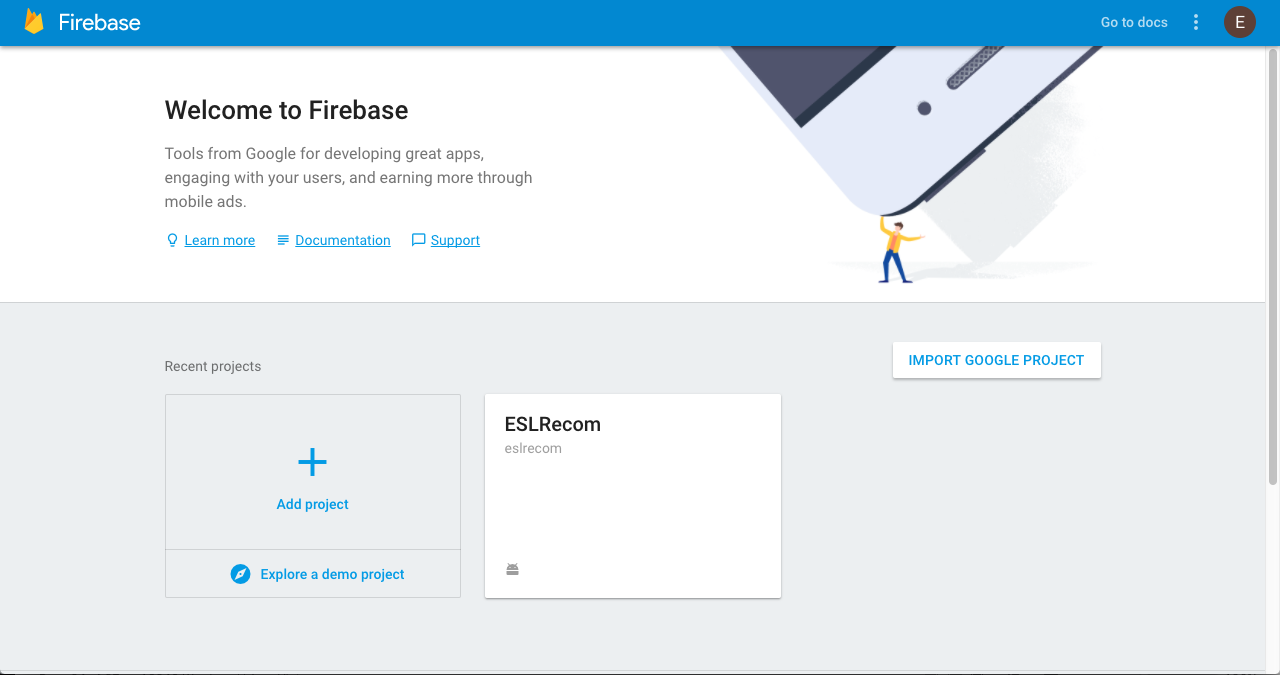
\includegraphics[scale=0.33]{afterlogin}
    \vskip 0.1in
	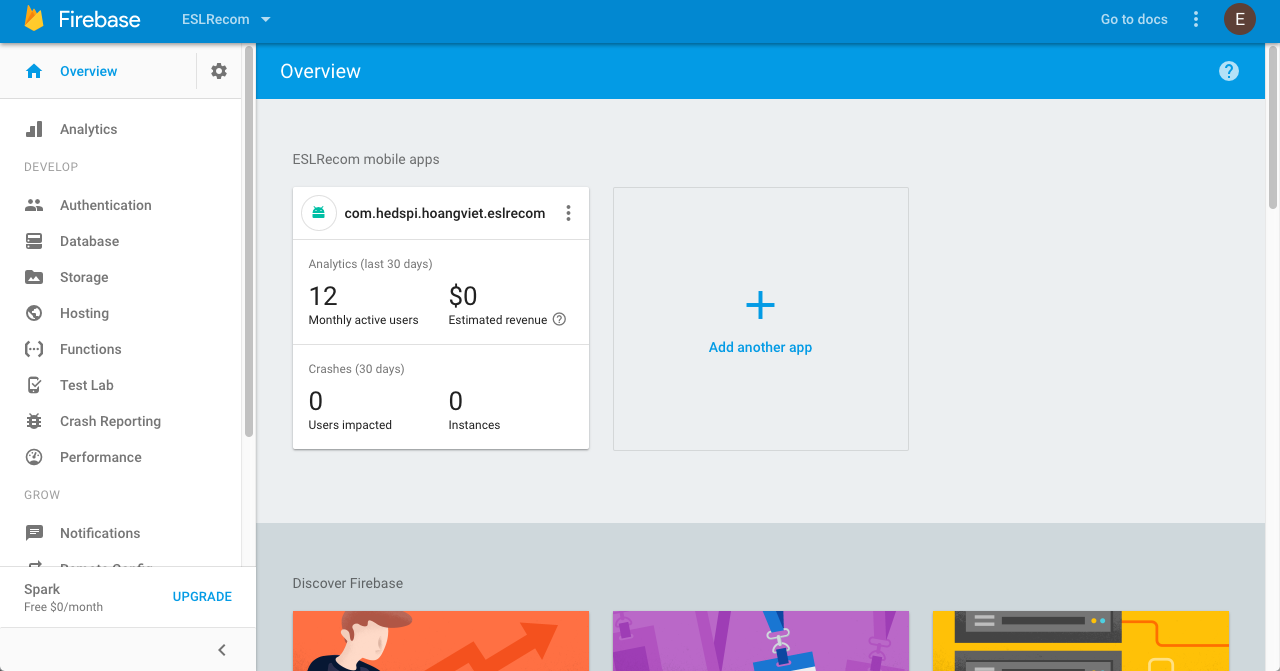
\includegraphics[scale=0.33]{consoledashboard}
    \caption{Giao diện console Firebase}
    \label{FirebaseAfterLogin}
  \end{center}
\end{figure}
	\item [] Trong hệ thống đề tài xây dựng, chúng ta quan tâm đến 3 mục sau :
	\item \textbf{Mục Analytic: }Quản lý các thông số sử dụng trên các thiết bị kết nối đến Firebase như số lượng người dùng active theo tháng, lợi nhuận thu được, event tương tác với người dùng..v..v... 
	\item \textbf{Mục Authentication: }Quản lý xác thực người dùng, thông tin người dùng đã đăng nhập, bao gồm \textit{email, số điện thoại, lần đăng nhập cuối cùng, uid...v..v...} sẽ được lưu trữ ở đây. 
	\vskip 0.1in
	\item []Người quản trị có thể thực hiện các thao tác quản trị: \begin{itemize}
	\item Thêm mới người dùng, reset mật khẩu, xoá người dùng đang tồn tại.
	\item Thay đổi cách thức đăng nhập : Bật/vô hiệu hoá đăng nhập qua Email/Password, Google, Facebook, ..v..v...
	\item Tạo email kích hoạt tài khoản, email thay đổi password , thay đổi địa chỉ email theo template có sẵn.
	\item Các tuỳ chỉnh quản lý khác như: OAuth, giới hạn một email cho một tài khoản, giới hạn số tài khoản login từ một địa chỉ IP..v..v...\\ \begin{figure}[H]
  \begin{center}
    %\leavevmode
	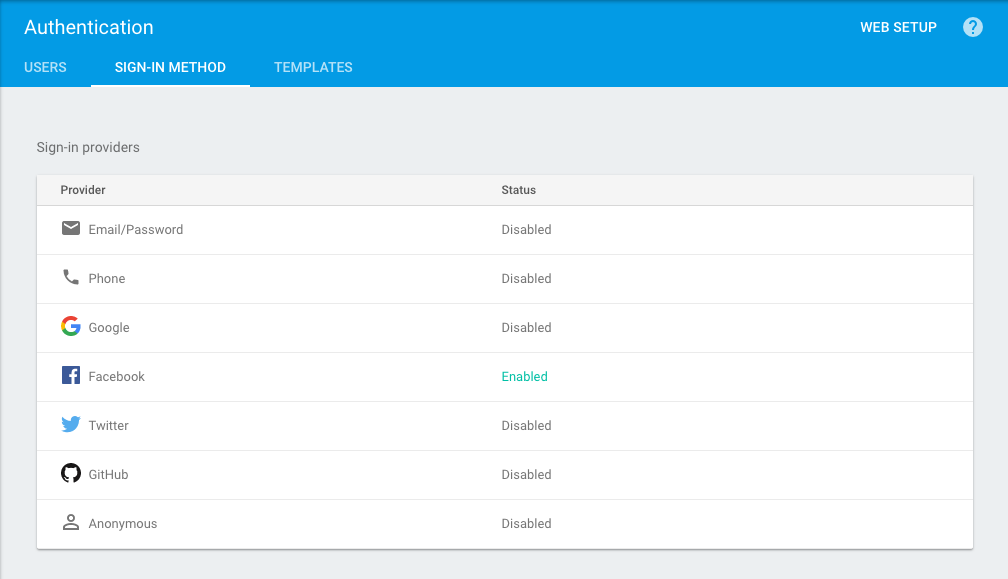
\includegraphics[scale=0.45]{firebase_authentication}
    \caption{Giao diện quản lý authentication}
    \label{FirebaseAuthentication}
  \end{center}
\end{figure}
	\end{itemize}
	\pagebreak
	\item \textbf{Mục Database: }Quản lý cơ sở dữ liệu thời gian thực, tất cả dữ liệu được lưu trữ ở định dạng JSON và với bất kể một sự thay đổi dữ liệu nào thì có sự phản hồi ngay lập tức, hiển thị đồng bộ. 	
	\vskip 0.1in
	\item []Người quản trị có thể thực hiện các thao tác quản trị: \begin{itemize}
			\item Thêm mới, thay đổi và xoá dữ liệu.
			\item Thiết lập tập luật giới hạn quyền truy cập dữ liệu đối với từng đối tượng người dùng khác nhau.
			\item Cấu hình tự động backup dữ liệu định kì
			\item Quan sát thông số sử dụng được Firebase thống kê\\ \begin{figure}[H]
  \begin{center}
    %\leavevmode
	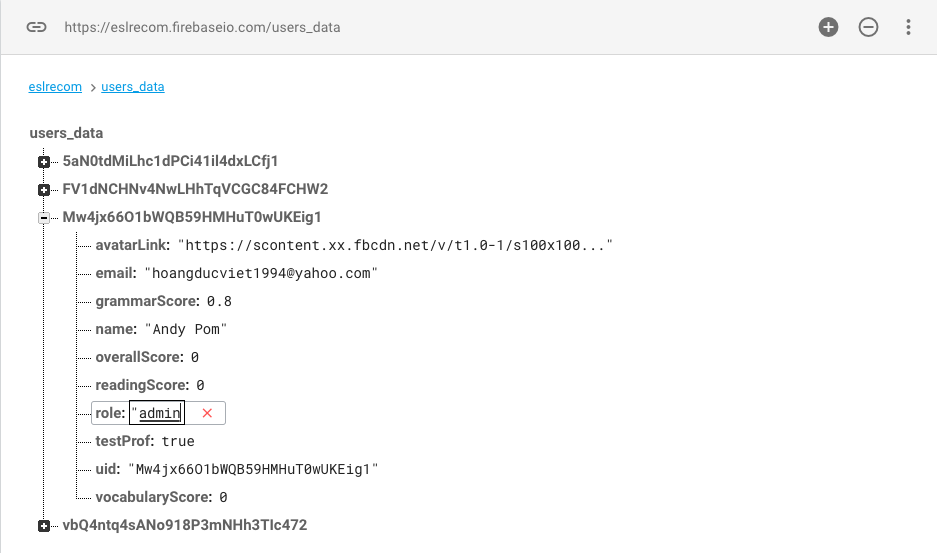
\includegraphics[scale=0.45]{firebase_database}
    \caption{Giao diện quản lý database}
    \label{FirebaseDatabase}
  \end{center}
\end{figure}
	\end{itemize}
\end{itemize}

{\Large \textbf{Tích hợp Firebase vào hệ thống }}\\

\textbf{Yêu cầu về môi trường:}
\begin{itemize}
	\item Điện thoại cài đặt Android 4.0 trở lên
	\item Google Play SDK, cài đặt qua Android SDK Manager
	\item Android Studio phiên bản mới nhất, v1.5 trở lên.\\ 
\end{itemize}
\pagebreak

\textbf{Cài đặt SDK}

Để sử dụng các thư viện Firebase cung cấp, người dùng cần thực hiện các thao tác sau đây:
\begin{itemize}
	\item Mở file \textcolor{pgrey}{build.gradle} của root và thêm vào google-services plugin:
	\begin{lstlisting}[frame=single, style=javacode, breaklines=true]
buildscript {
    // ...
    dependencies {
        // ...
        classpath 'com.google.gms:google-services:3.1.0'
    }
}	

	\end{lstlisting}
	\item Sau đó, mở file \textcolor{pgrey}{build.gradle} của app và thêm vào:
	\begin{lstlisting}[frame=single, style=javacode, breaklines=true]
apply plugin: 'com.android.application'

android {
  // ...
}

dependencies {
  // ...
  compile 'com.google.firebase:firebase-core:10.2.6'
  
  // Getting a "Could not find" error? Make sure you have
  // the latest Google Repository in the Android SDK manager
}

// ADD THIS AT THE BOTTOM
apply plugin: 'com.google.gms.google-services' 

	\end{lstlisting}

\end{itemize}

\textbf{Sử dụng:}

\begin{itemize}
	\item Lưu trữ dữ liệu offline trên ổ đĩa và đồng bộ khi có thể .\begin{lstlisting}[frame=single, style=javacode, breaklines=true]
FirebaseDatabase.getInstance().setPersistenceEnabled(
true);
FirebaseDatabase.getInstance().getReference()
.keepSynced(true);

	\end{lstlisting}
	\pagebreak
	\item Để thêm dữ liệu vào database:
	\begin{lstlisting}[frame=single, style=javacode, breaklines=true]
private DatabaseReference mDatabase;

mDatabase = FirebaseDatabase.getInstance().getReference();
DatabaseReference mRef = mDatabase.getReference("copyright");

mRef.setValue("testing");

	\end{lstlisting}

	\item Lấy dữ liệu từ trên Firebase xuống:\begin{lstlisting}[frame=single, style=javacode, breaklines=true]
mDatabase.child(userId).addValueEventListener(new ValueEventListener() {
    @Override
    public void onDataChange(DataSnapshot dataSnapshot) {

        User user = dataSnapshot.getValue(User.class);

        Log.d(TAG, "User name: " + user.getName() + ", email " + user.getEmail());
    }

    @Override
    public void onCancelled(DatabaseError error) {
        // Failed to read value
        Log.w(TAG, "Failed to read value.", error.toException());
    }
});

	\end{lstlisting}
\end{itemize}
